% To je predloga za poročila o domačih nalogah pri predmetih, katerih
% nosilec je Blaž Zupan. Seveda lahko tudi dodaš kakšen nov, zanimiv
% in uporaben element, ki ga v tej predlogi (še) ni. Več o LaTeX-u izveš na
% spletu, na primer na http://tobi.oetiker.ch/lshort/lshort.pdf.
%
% To predlogo lahko spremeniš v PDF dokument s pomočjo programa
% pdflatex, ki je del standardne instalacije LaTeX programov.

\documentclass[a4paper,11pt]{article}
\usepackage{a4wide}
\usepackage{fullpage}
\usepackage[utf8x]{inputenc}
\usepackage[slovene]{babel}
\selectlanguage{slovene}
\usepackage[toc,page]{appendix}
\usepackage[pdftex]{graphicx} % za slike
\usepackage{setspace}
\usepackage{color}
\definecolor{light-gray}{gray}{0.95}
\usepackage{listings} % za vključevanje kode
\usepackage{hyperref}
\renewcommand{\baselinestretch}{1.2} % za boljšo berljivost večji razmak
\renewcommand{\appendixpagename}{Priloge}

\lstset{ % nastavitve za izpis kode, sem lahko tudi kaj dodaš/spremeniš
language=Python,
basicstyle=\footnotesize,
basicstyle=\ttfamily\footnotesize\setstretch{1},
backgroundcolor=\color{light-gray},
}

\title{Optični pretok}
\author{David Rubin (david.rubin@student.um.si)}
\date{\today}

\begin{document}

\maketitle

\section{Implemetacija}

Algoritem sem implementiral v programskem jeziku Python. Za delovanje je potrebna knjižnica opencv, scipy, numpy in pa matplotlib (opcijsko za izrisovanje nekaterih informacij). Implementiran program povpraša po video datoteki, z zastavicami pa tudi lahko nastavimo določene parametre. Opisi posameznih parametrov so na voljo na sliki~\ref{img:prog_help}.

Rezultati programa so dosegljivi na povezavi \url{https://imgur.com/a/PDdIXaf}

\vspace{0.5cm}
Za ključne točke pri redkem pretoku sem uporabil Shi-Tomasi detektor na voljo v knjižnici opencv (\texttt{goodFeaturesToTrack}). Za odstranjevanje vpliva šuma na slikah jih pred zaznavanjem pretoka gladim z Gaussovim jedrom. Prav tako sem odstranil (zakomentiral) pogoje, ki narekujejo kdaj se naj izračuna pretok (lastne vrednosti so dovolj velike in razmerje med največjo in najmanjšo lastno vrednostjo je dovolj veliko). Razlog tišči v tem, da nisem zaznal bistvene izboljšave. Pri risanju gostega pretoka sem se odločil, da ga prikažem kot mrežo, torej pretok se poračuna za vsak posamezen piksel (znotraj okna), prikaže pa se v mreži s črtami. Pri redkem pretoku skušam ohraniti točke na objektu kateremu sledimo, prav tako pa izrisujem črto, ki prikazuje potovanje točke skozi čas. Pri večini primerov sem uporabil velikost okna 31, pri redkem pretoku pa za izbiro ključnih točk največ 100. Ključne točke se v vsakem koraku zmanjšujejo (prenehajo slediti) v kolikor ni pri njih zaznam optični pretok.

\begin{figure}
	\centering
	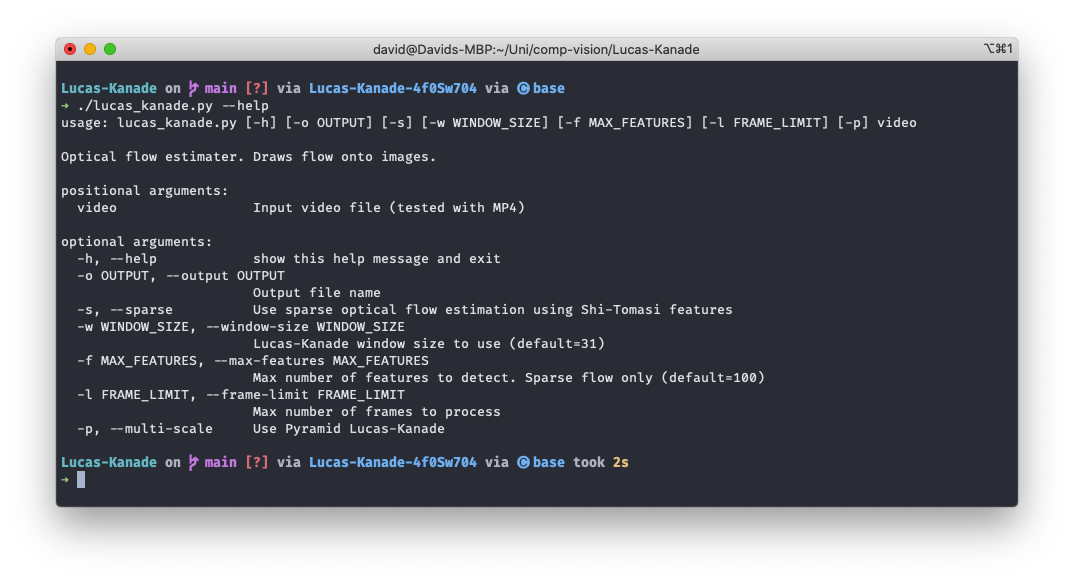
\includegraphics[width=1\textwidth]{images/prog_help}
	\caption{Meni za pomoč ob zagonu programa. Program obvezno potrebuje le video datoteko (preverjeno z MP4 datotekami).}
	\label{img:prog_help}
\end{figure}

\end{document}
